\chapter[Homes in Iceland]{
    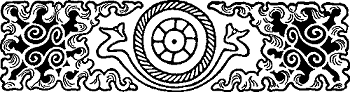
\includegraphics[width=9.3cm]{viking-tales/035}\\
    Homes in Iceland}

\lettrine{M}{en} had been feasting in Ingolf's house. But there was no
laughing and no shouting of jokes. Ingolf sat in his high seat frowning
and gloomy. His head hung on his breast. He was staring into the fire.
Now he raised his head and looked about the hall.

``Comrades,'' he said, ``what shall we do? Herstein and Holmstein died
by our swords. Their kinsmen hunger to kill us. Besides, when Harald
hears of our deed, there will not be a safe place in Norway for us. He
will never let a man fight out an honest quarrel. Where shall we go?''

A man stood up from the bench.

``We have friends in the Shetlands,'' he said. ``Let us find homes
there.''

Then Leif, in the high seat opposite Ingolf, stood up.

``No, not the Shetlands, my foster-brother.\footnote{See note about
foster-brothers on page~\pageref{foster-brothers}.} They are crowded
already. Besides, Harald will not long keep his hands off them. Then they
will be no better than Norway. England and Ireland and Scotland are old.
My eyes ache for something new. What of that far island that Floki found?
It is empty. We could choose our land from the whole country. There is
good fishing. There are green valleys. And Butter Thorolf says that
butter drops from every weed. There are mountains and deserts where we
may find adventure. I say, let us steer for Iceland!''

When he stopped, many of the men shouted:

``Yes! Iceland!''

But an old man stood up.

``We have all laughed at that tale of Butter Thorolf's,'' he said. ``But
Floki himself said that the sea about the island is full of ice that
pushes upon the land, that no ship can live in that water in the winter,
that great mountains of ice cover the island. Did not all his cattle die
there of hunger and cold, and did he not come back to Norway cursing
Iceland?''

``Oh, Sighvat, you are old and fearful,'' called out Leif, and he
laughed.

Then he stretched himself up and threw back his head.

``Are we afraid of ice? Have we not seen angry water before? I have been
hungry, but I have never died of it. Surely if there are fish in the sea
and grass in the valleys, we can live there. I should like to stand on a
hill and look around on a wide land and think, `This is all ours,' and
out upon a rough sea and think, `Far off there are our foes and they
dare not come over to us.' Besides, we shall have no Shockhead Harald to
lord it over us. We can come and go and feast and fight as we please. We
shall be our own kings. And our ships will be always waiting to take us
away, when we are weary of it. And we shall see things that other men
have never seen. I am tired of the old things. Perhaps in after days men
will make songs about `those foster-brothers, Ingolf and Leif, who made
a new country in a wonderful land, and whose sons and grandsons are
mighty men in Iceland!'''

Ingolf leaped up from his chair.

``By the strong arm of Thor!'' he cried, ``I like the sound of it. Now I
make my vow.''

He raised his drinking-horn.

``I vow that I will find this Iceland and pass the winter there, and
that if man can live upon it I will go back there and set up my home.''

``And I vow that I will follow my foster-brother,'' cried Leif.

And many men vowed to go.

So on the next day they began to make ready a boat. They looked her over
carefully and recalked every seam and freshly painted her and put into
her their strongest oars and made her a new sail.

``This will be the longest voyage that she ever made,'' Ingolf said.

When the work was done, they put into her great stores, axes, hammers,
fish-nets, cooking-kettles, kegs of ale, chests of hard bread, chests of
smoked meat, brass kettles full of flour, skin bottles of water. They
stowed these things away in the ends of the ship. When they were ready
they put in four head of cattle.

``We shall need the milk and perhaps the meat,'' Ingolf said.

Many men wished to go, but Ingolf had said:

``There is little room to spare and little food and drink. I have
planned for half a year. But perhaps we must be sailing longer than
that. Our food may run short. We must not have extra mouths to feed.
There are thirty oars in our boat. I will take only one man for every
oar, and Leif and I will steer.''

So they started off. Leif stood in the prow leaning forward and looking
far ahead, and he sang:

\begin{quote}
``What does the swimming dragon smell?\\
A stormy sea, an empty land,\\
Hunger, darkness, giants, fire.\\
Leif and his sword do laugh at that.''
\end{quote}

They sailed for days and saw no land. Sometimes they passed ships and
always made sure to sail close enough to hail them.

``Where are you going?'' Ingolf would call.

``To Norway,'' would come back the answer.

``For trade or fight?'' Leif would shout.

Then would ring out a great laugh from that boat and this answer:

``A shut mouth is a good friend.''

So the two ships sailed on, and the men were glad to have heard a
greeting and to have called one.

But at last there were the Shetlands.

``We will go in here and rest,'' Ingolf said.

When they rowed to shore a certain Shetland man stood there. He watched
them land and looked them all over. Then he walked up to Ingolf and
said:

``You look like brave men. Welcome to Shetland. You shall come to my
house and rest your legs from ship-going and fill your stomachs. I
hunger for news of Norway.''

So they went to his house and stayed there for three days. And good it
seemed to be near a fire and in a quiet bed and before a steaming
platter. When they went to the shore to start off again, the Shetland
man had his thralls carry a keg of ale and a great kettle of cooked meat
and put them into the ship.

``Think of me when you eat this,'' he said.

Then the Norsemen put to sea again and sailed for a long time.

One day a terrible storm came up; the sky was black; the wind howled
through the ship. Great waves leaped in the sea.

``Down with the sail and out with the oars!'' Ingolf shouted.

So the men furled the sail and took down the mast and laid it along the
bottom of the boat. As they worked, one man was washed overboard and
drowned. The men sat down to row, but the tumbling waves tossed the boat
about and poured over her and broke three of the oars. But still the men
held on. They were wet to the skin and were cold, and their arms and
legs ached with the hard work, and they were hungry from the long
waiting, but not one face was white with fear.

``Ran, in her caves under sea, wants us for company to-night,'' Ingolf
laughed.

So they tossed about all night, but in the morning the wind died down.
Great waves still rolled, and for days the sea was rough, but they could
put up the sail. Then one day Leif, as he sat in the pilot's seat,
jumped to his feet and sang:

\begin{quote}
``To eyes grown tired with looking far,\\
All at once appeared an island,\\
A stretching-place for sea-legs,\\
A quiet bed for backs grown stiff\\
On rowing-bench on rolling sea.\\
A place to build a red fire\\
And thaw the blood that sea-winds froze.''
\end{quote}

But when they came near they saw no place to land. The island was like a
mountain of rock standing out of the water. The sides were steep and
smooth. They sailed around it, but found no place to climb up.

``There are many other islands here,'' said Leif. ``We will try
another.''

So he steered to another. It, too, was a steep rock, but one side sloped
down to the water and was green with grass.

``Oh, I have not seen anything so good as that green grass since I
looked into my mother's face,'' one man said.

There was a little harbor there. The men rowed in and quickly jumped out
and put the rollers under the ship and pulled her upon shore. Then they
threw themselves down on the grass and rolled and stretched their arms
and shouted for joy. After that they built a fire and warmed themselves
and cooked a meal and ate like wolves. They slept there that night.

In the morning before Ingolf's men started away they were standing high
up on the hillside, looking about. They saw no houses on any of the
islands, but they saw smoke rise from one hillside.

``Some other men, like us, weary of the sea and stopping to rest,'' said
Ingolf.

They saw the island that they had sailed around the night before.

``There can surely be nothing but birds' nests on top of that,'' Sighvat
said.

``Look!'' cried another, pointing.

Men were standing on the flat top of that island. They were letting a
boat down the steep side with ropes. When it struck the water, they made
a rope fast to the rock and slid down it into the ship and sailed off.

``Some robber vikings from Scotland or Ireland,'' laughed Leif. ``It is
a good hiding place for treasure.''

Soon Ingolf and his men got into their ship and were off. Old Sighvat
grumbled.

``Is this land not new enough and empty enough and far enough? I am
tired of sea, sea, sea, and nothing else.''

``We started for Iceland,'' said Ingolf, ``and I will not stop before I
come there. I have a vow. Did you make none, Sighvat?''

Then they were on the water again for weeks with no sight of land.

``Oh! I would give my right hand to see a dragon pawing the water off
there and to fling a word to its men,'' Sighvat said.

``No hope of that,'' replied Ingolf. ``Only three dragons before ours
have ever swept this water, and men are not sailing this way for
pleasure or riches.''

So only the desolate sea stretched around them. Sometimes it was smooth
and shining under the sun. Often it was torn by winds, and a gray sky
hung over it, and the men were drenched with rain. Once they ran into a
fog. For three days and nights they could not see sun or stars to steer
by. They forgot which way was north. When after three days the fog
lifted, they found that they had been going in the wrong direction, and
they had to turn around and sail all that weary way over again. But at
last one afternoon they saw a white cloud resting on the water far off.
As they sailed toward it, it grew into long stretches of black, hilly
shore with a blue ice mountain rising from it. The sun was going down
behind that mountain, and long lines of pink and of shining green, and
great purple shadows streaked the blue.

``It is Iceland!'' shouted the men.

``It is like Asgard the Shining,'' Ingolf said.

But it was still far off. Men can see a long way there because the air
is so clear. So Ingolf and his people sailed on for hours and at last
came into a harbor. A little green valley sloped up from it. On one side
was the bright ice mountain. Back of it were bare black and red hills.
In that valley Ingolf and his men drew up their boat and camped. At
supper that night one of the men said:

``I almost think I never felt a fire before or had warm food in my
mouth.''

The men laughed.

``It is four months since we left Norway,'' Ingolf said. ``Few men have
ever been on the sea so long.''

That night they put up the awning in the boat and slept under it.

After that some men went fishing every day in the rowboat that they had.
And Ingolf took others, and they sailed along the shore, seeing what
kind of a land this was. But winter began to come on. Then Ingolf said:

``Remember what Floki said of the ice and the rough sea in winter. Soon
we cannot sail any longer. Let us choose a place to stay and build a hut
there and cut hay for our cattle.''

So they did. Their hut was a little mean thing of stones and turf. They
kept the cattle and the hay in it. Sometimes they slept there, when it
was very cold. But most of the time they ate and slept by a great
bonfire out of doors where it was clean. Leif said:

``I like the cold air of the sea better than the bad-smelling air of a
house, even though it is warm.''

Now every day Ingolf and Leif and some of the men walked about the
island. At night they all sat around the campfire and talked of what
they had seen during the day.

``This is surely a wonderful land,'' Ingolf said once. ``It is at the
same time like Niflheim and like Asgard. Here is a spot green and soft,
a sweet cradle for men. Next it is a mountain of ice where men would
freeze to death. And next to that is a hill of rock that seems to have
come out of some great fire. Yesterday I saw a cave on the seashore. The
door of it was big enough for a giant. The waves broke at the doorstep.
A terrible roaring came from the cave. I think it is the home of a
giant. I think that giants of fire and giants of frost made this island.
I have seen great basins in the rocks filled with warm water. They
looked like giants' bath-tubs. I have seen boiling water shoot up out of
the ground. I have walked, and have felt and heard a great rumbling
under me as though some giant were sleeping there and turning over in
his sleep. One day I stood on a mountain and looked inland. There was a
wide desert of sand and black and red rock with nothing growing on it.
The fierce wind blew dirt into my eyes, and the cold of it froze the
marrow in my bones. When I have seen these things I have cursed the
country, and have said: `The gods hate Iceland. I will not stay here.'
But then I have walked through beautiful warm valleys where the winds
did not come. I saw in my mind the flowers that we found last summer. I
saw our cattle feeding on the sweet grass. I thought of the sea full of
good fish. I saw my house built among green fields, and my wife sitting
in her home, and my children playing among the flowers and making up
tales about the bright ice mountains. I saw the wide, rough seas between
me and Harald and our foes. Then I thought to myself, `It is the
sweetest home on earth.' As for me, I am coming here to live. What do
you say, comrades?''

``Have I not vowed to follow you, foster-brother?'' said Leif. ``And
indeed I never saw a land that I liked better. I don't believe in your
giants. My sword is my god, and my ship is my temple, and I like this
land to set them up in.''

They sat about the fire long that night making plans.

``You shall go home and get our women and our things, Ingolf,'' said
Leif. ``I will off to Ireland and have a frolic. There will be little
play of swords in this empty land, and I want to have one last game
before I hang up my battle-knife. Besides, I will come to you with a
ship full of gold and clothes and house-hangings such as we cannot get
here, and they will cost me nothing but the swing of a sword.''

As they talked, Ingolf looked up at the sky. The northern lights were
quivering there. They were like great flames of yellow and green and
red.

``See,'' he said, and pointed. ``We are not so far that the gods will
forget us. There is the flash of the armor of the Valkyrias.\footnote{See
note about Valkyrias on page~\pageref{valkyrias}.} A battle is on
somewhere, and Odin has sent his maidens to choose the heroes for
Valhalla.''

Leif only laughed and lay down to sleep.

So in the spring they all went back to Norway. Leif got ready the boat
again and merrily sailed for Ireland.

``Here I go to get riches for our new land,'' he said.

Ingolf set his men to cutting down pines in the forest and some to
building a new ship. He had his thralls plant large crops of grain and
grind flour and make new kegs and chests of wood. He himself worked much
at the forge, making all kinds of tools--spades, axes, hammers,
hunting-knives, cooking kettles. The women were busy weaving and sewing
new clothes. Ingolf sold his house and land and everything that he could
not take with him.

After about two years Leif came back. He had ten thralls that he had got
in Ireland. He took Ingolf aboard his ship and raised the covers of
great chests. Gold helmets, silver-trimmed drinking-horns, embroidered
robes, and swords flashed out.

``Did I not say that I would come back with a full ship?'' he laughed.

At last all things were ready for starting.

``To-day I will sacrifice to Thor and Odin,'' Ingolf said. ``If the
omens are good we will start to-morrow.''

``Well, go, foster-brother,'' laughed Leif. ``But I have better things
to do. I will be putting the cattle into the ship and will have all
ready.''

So Ingolf and his men went into the forests a little way. There in a
cleared space stood a large building. In front of this temple the men
killed two horses for Odin. Ingolf caught some of the blood in a brass
bowl. He raised it and looked up at the sky and said:

``All-wise and all-father Odin, and Thor who loves the thunder, I give
these horses to you. Tell me whether it is your will that we go to
Iceland.''

As he said that, a raven flew over his head. Ingolf watched it.

``It is Odin's will that we go,'' he said. ``He sent his raven\footnote{
See note about Odin's ravens on page~\pageref{odins-ravens}.} to tell us.
It is flying straight toward Iceland.''

The men shouted with joy at that.

Now they hung some of the meat of the horses on a tree near the temple.

``For the ravens of Odin,'' they said.

Ingolf carried the bowl of blood into the temple. He went through the
feast hall in front to a little room at the back. Here stood wooden
statues of the gods in a semicircle. Before them was a stone altar.
Ingolf took a little brush of twigs that lay on it and dipped it into
the blood and sprinkled the statues.

``You shall taste of our sacrifice,'' he said. ``Look kindly on us from
your happy seats in Asgard.''

Then they went into the feast hall. There thralls were boiling the
horseflesh in pots over the fire. The tables were standing ready before
the benches. Ingolf walked to the high seat. All the others took their
places at the benches. When the horns came round, Ingolf made this vow:

``I vow that I will build my house wherever these pillars lead me.''

He put his hand upon a tall post that stood beside the high seat. There
was one at each side. They were the front posts of the chair. But they
stood up high, almost to the roof. They were wonderfully carved and
painted with men and dragons. On the top of each one was a little statue
of Thor with his hammer.

At the end of the feast Ingolf had his thralls dig these pillars up. He
had a little bronze chest filled with the earth that was under the
altar.

``I will take the pillars of my high seat to Iceland,'' he said, ``and I
will set up my altar there upon the soil of Norway, the soil that all my
ancestors have trod, the soil that Thor loves.''

So they carried the pillars and the chest of earth and the statues of
the gods, and put them into Ingolf's boat.

``It is a well-packed ship,'' the men said. ``There is no spot to
spare.''

Tools, and chests of food, and tubs of drink, and chests of clothes, and
fishing nets were stowed in the bows of both boats. In the bottom were
laid some long, heavy, hewn logs.

``The trees in Iceland are little,'' Ingolf said. ``We must take the
great beams for our homes with us.''

Standing on these logs were a few cattle and sheep and horses and pigs.
The rowers' benches were along the sides. In the stern of each boat was
a little cabin. Here the women and children were to sleep. But the men
would sleep on the timbers in the middle of the boat and perhaps they
would put up the awning sometimes.

At last everyone was aboard. Men loosed the rope that held the boats.
The ships flashed down the rollers into the water, and Ingolf and Leif
were off for Iceland. As they sailed away everyone looked back at the
shore of old Norway. There were tears in the women's eyes. Helga, Leif's
wife, sang:

\begin{quote}
``There was I born. There was I wed.\\
There are my father's bones.\\
There are the hills and fields,\\
The streams and rocks that I love.\\
There are houses and temples,\\
Women and warriors and feasts,\\
Ships and songs and fights--\\
A crowded, joyous land.\\
I go to an empty land.''
\end{quote}

There was the same long voyage with storm and fog. But at last the
people saw again the white cloud and saw it growing into land and
mountains. Then Ingolf took the pillars of his high seat and threw them
overboard.

``Guide them to a good place, O Thor!'' he cried.

The waves caught them up and rolled them about. Ingolf followed them
with his ship. But soon a storm came up. The men had to take down the
sails and masts, and they could do nothing with their oars. The two
ships tossed about in the sea wherever the waves sent them. The pillars
drifted away, and Ingolf could not see them.

``Remember your pillars, O Thor!'' he cried.

Then he saw that Leif's ship was being driven far off.

``Ah, my foster-brother,'' he thought, ``shall I not have you to cheer
me in this empty land? O Thor, let him not go down to the caves of Ran!
He is too good a man for that.''

On the next day the storm was not so hard, and Ingolf put in at a good
harbor. A high rocky point stuck out into the sea. A broad bay with
islands in the mouth was at the side. Behind the rocky point was a level
green place with ice-mountains shining far back.

After a day or two Ingolf said:

``I will go look for my pillars.''

So he and a few men got into the rowboat and went along the shore and
into all the fiords, but they could not find the pillars. After a week
they came back, and Ingolf said:

``I will build a house here to live in while I look for the posts. This
way is uncomfortable for the women.''

So he did. Then he set out again to look for the pillars, but he had no
better luck and came back.

``I must stay at home and see to the making of hay and the drying of
fish,'' he said. ``Winter is coming on, and we must not be caught with
nothing to eat.''

So he stayed and worked and sent two of his thralls to look for the holy
posts. They came back every week or two and always had to say that they
had not found them. Midwinter was coming on.

\begin{figure}[ht]
    \centering
    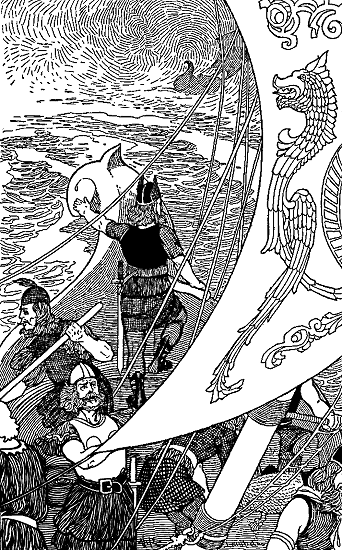
\includegraphics[width=9.1cm]{viking-tales/036}
    \caption{``Then he saw that Leif's ship was being driven afar off''}
\end{figure}

``Ah!'' said Ingolf's wife one day, ``do you remember the gay feast that
we had at Yule-time? All our friends were there. The house rang with
song and laughter. Our tables bent with good things to eat. Walls were
hung with gay draperies. The floor was clean with sweet-smelling
pine-branches. Now look at this mean house; its dirt floor, its bare
stone walls, its littleness, its darkness! Look at our long faces. No
one here could make a song if he tried. Oh! I am sick for dear old
Norway.''

``It is Thor's fault,'' Ingolf cried. ``He will not let me find his
posts.''

He strode out of the house and stood scowling at the gray sea.

``Ah, foster-brother!'' he said. ``It was never so gloomy when you were
by my side. Where are you now? Shall I never hear your merry laugh
again? That spot in my palm burns, and my heart aches to see you. That
arch of sod keeps rising before my eyes. Our vows keep ringing in my
ears.''

At last the long, gloomy winter passed and spring came.

``Cheer up, good wife,'' Ingolf said. ``Better days are coming now.''

But that same day the thralls came back from looking for the posts.

``We have bad news,'' they said. ``As we walked along the shore looking
for the pillars we saw a man lying on the shore. We went up to him. He
was dead. It was Leif. Two well-built houses stood near. We went to
them. We knew from the carving on the door-posts that they were Leif's.
We went in. The rooms were empty. Along the shore and in the wood back
of the house we found all of his men, dead. There was no living thing
about.''

Ingolf said no word, but his face was white, and his mouth was set. He
went into the house and got his spears and his shield and said to his
men:

``Follow me.''

They put provisions into the boat and pushed off and sailed until they
saw Leif's houses on the shore of the harbor. There they saw Leif and
the men who were his friends, dead. Their swords and spears were gone.
Ingolf walked through the houses calling on Helga and on the thralls,
but no one answered. The storehouse was empty. The rich hangings were
gone from the walls of the houses. There was nothing in the stables. The
boat was gone.

Ingolf went out and stood on a high point of land that jutted out into
the water. Far along the coast he saw some little islands. He turned to
his men and said:

``The thralls have done it. I think we shall find them on those
islands.''

Then he went back to Leif and stood looking at him.

``What a shame for so brave a man to fall by the hands of thralls! But I
have found that such things always happen to men who do not sacrifice to
the gods. Ah, Leif! I did not think when we made those vows of
foster-brotherhood that this would ever happen. But do not fear. I
remember my promise. I had thought that a man's blood is precious in
this empty land, but my vow is more precious.''

Now they laid all those men together and tied on their hell-shoes.

``I need my sword for your sake, foster-brother. I cannot give you that.
But you shall have my spears and my drinking-horn,'' said Ingolf. ``For
surely Odin has chosen you for Valhalla, even though you did not
sacrifice. You are too good a man to go to Niflheim. You would make
times merry in Valhalla.''

So Ingolf put his spears and his drinking-horn by Leif. Then the men
raised a great mound over all the dead. After that they went aboard
their boat and sailed for the islands that Ingolf had seen. It was
evening when they reached them.

``I see smoke rising from that one,'' Ingolf said, pointing.

He steered for it. It was a steep rock like that one in the Faroes, but
they found a harbor and landed and climbed the steep hill and came out
on top. They saw the ten thralls sitting about a bonfire eating. Helga
and the other women from Leif's house sat near, huddled together, white
and frightened. One of the thralls gave a great laugh and shouted:

``This is better than pulling Leif's plow. To-morrow we will sail for
Ireland with all his wealth.''

``To-morrow you will be freezing in Niflheim,'' cried Ingolf, and he
leaped among them swinging his sword, and all his men followed him, and
they killed those thralls.

Then Ingolf turned to Helga. She threw herself into his arms and wept.
But after a while she told him this story:

``When springtime came, Leif thought that he would sow wheat. He had but
one ox. The others had died during the winter. So he set the thralls to
help pull the plow. I saw their sour looks and was afraid, but Leif only
laughed:

`\,``What else can thralls expect?' he said. `Never fear them, good wife.'

``Now one day soon after that the thralls came running to the house
calling out:

`\,``The ox is dead! The ox is dead!'

``Leif asked them about it. They said that a bear had come out of the
woods and killed it, and that they had scared the beast away. They
pointed out where it had gone. Then Leif called his men and said:

`\,``A hunt! I had not hoped for such great sport here. Ah, we will have a
feast off that bear!'

``So they took their spears and went out into the woods. As soon as they
were gone, the thralls came running into the house and took down all the
swords and shields from the wall and ran out. In some way they met my
lord and his men in the woods and killed them. Then they came back and
took everything in the house and dragged us to the boat and sailed
here.''

``O my brother!'' said Ingolf, ``where is that song about `those two
foster-brothers, Ingolf and Leif, who made a new country in a wonderful
land, and whose sons and grandsons are mighty men in Iceland'? But come
home with me, Helga.''

So they took the women and Leif's things and Leif's boat and sailed
home. The next day after they came to Ingolf's house, Helga said:

``We have made your family larger, brother Ingolf. Will you not take
Leif's two houses and live in them? He does not need them now. He would
like you to have them.''

``It would be pleasant to live there,'' Ingolf said. ``I thank you.''

So the next day they loaded everything aboard the two ships and sailed
for Leif's house. There they stayed for a year. Ingolf still sent his
thralls out to look for the pillars. He was careful always to have hay,
so his cattle prospered. That spring he planted wheat, but it did not
grow well.

``This is sickly stuff,'' Ingolf said. ``It takes too much time and
work. It is better to save the land for hay. Perhaps we can sometime go
back to Norway for flour.''

At last one day the thralls came home and said:

``We have found the pillars.''

Ingolf jumped to his feet. He cried out:

``You have kept me waiting three years, Thor. But as soon as my house
and temple are built, I will sacrifice to you three horses as a
thank-offering.''

``It is a long way off, master,'' the thralls said, ``and we have found
much better places in our walks about the island.''

``Thor knows best,'' Ingolf answered. ``I will settle where he leads
me.''

So that summer they loaded everything into the ships again and sailed
west along the coast until they came to the place where the pillars
were. The land there was low and green. On both sides were low hills. A
little lake glistened back from shore. In the valley were hot springs,
with steam rising from them.

``It looks like smoke,'' the men said. ``It is very strange to see hot
water and smoke come out of the ground.''

In front of this green land was a good harbor with islands in it. Far
over the sea toward the north shone a great ice-mountain.

``I like the place,'' Ingolf said. ``I will make this land mine.''

So he built fires at the mouth of the river near there, and stood by
them and called out loudly:

``I have put my fire at the mouth of these rivers. All the land that
they drain is mine, and no man shall claim it but me. I will call this
place Reykjavik.''\footnote{See note about Reykjavik on
page~\pageref{reykjavik}.}

Then Ingolf built his feast hall. He himself carved the beams and the
door-posts. Gaily painted dragons leaned out from the doors and stood up
from the gables. Men and animals fought on the door-posts. For the doors
he made at the forge great iron hinges. Their ends curved and spread all
over the door. Near his feast hall he built a storehouse and a kitchen
and a smithy and a stable and a bower for the women.

``We do not need a sleeping-house for guests,'' he said. ``Who would be
our guests?''

He roofed all his buildings with turf. It made them look like green
mounds with gay carved and painted walls under them. He built also a
temple, and on that was beautiful carving. In this he set up those
statues that had been in his old temple. He put up, too, those pillars
of his high seat that had been drifting about so long. Under them he
laid the soil of Norway that he had brought in the little bronze chest.

``I have kept my vow, O Thor!'' he cried.

Then he sacrificed three horses that he had promised to Thor. After that
was over, he said:

``Here is a good field for sport. Let us have some of the old games that
we used to play at home. Who will wrestle with me?''

So they wrestled there and ran races and swam in the water. The women
sat and looked on.

``Oh, this is good to see!'' Helga cried. ``We are as gay as we used to
be in old Norway.''

But it was not many weeks before Ingolf said:

``I wish that I might sometime see sails in that harbor. I wish that I
might think, `Around this point of land is another farm, and across the
bay is another. I can go there when I am very lonely.' I wish that I
might sometime be invited to a feast. I wish that I might sometimes hear
the good, clanging music of weapons at play. It is a good land, but we
have lived alone for four years. I am hungry for new faces and for
tidings of Norway.''

One night as he and his men sat about the long fire in the feast hall, a
servant threw a great piece of wood upon the fire. It was streaked with
faded paint and it showed bits of carving.

``See,'' said Ingolf, pointing to it, ``see what is left of a good
ship's prow! What lands have you seen, O dragon's head? What battles
have you fought? What was your master's name? Where did the storm meet
you? Perhaps he was coming to Iceland, comrades. Would it not have been
pleasant to see his sail and to shake his hand and to welcome him to
Iceland? But instead he is in Ran's caves, and only his broken prow has
drifted here.''

Now it was not many months after that when one of the men came running
into the feast hall, shouting:

``A sail! a sail in the harbor!''

All those men gave a shout with no word in it, as though their hearts
had leaped into their throats. They jumped up and ran to the shore and
stood there with hungry eyes. When the men landed, those Icelanders
clapped them on the shoulders, and tears ran down their faces. For a
long time they could say nothing but ``Welcome! Welcome!''

\begin{figure}[ht]
    \centering
    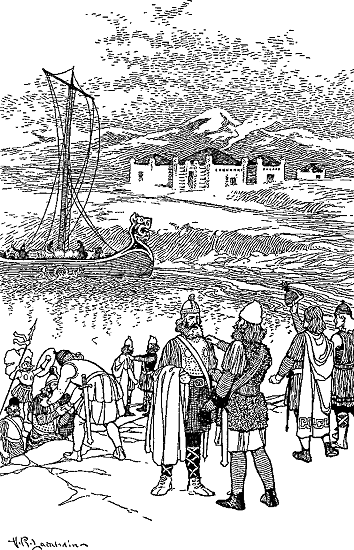
\includegraphics[width=9.1cm]{viking-tales/037}
    \caption{``Those Icelanders clapped them on the shoulders''}
\end{figure}

But after a while Ingolf led them to the feast hall and had a feast
spread at once. While the thralls were at work, the men stood together
and talked. Such a noise had never been in that hall before.

``We have already built our fires and claimed our land up the shore a
way,'' the leader said. ``Men in Norway talk much of Ingolf and Leif,
and wonder what has happened to them.''

Then Ingolf told them of all that had come to pass in Iceland; and then
he asked of Norway.

``Ah! things are going from bad to worse,'' the newcomers said. ``Harald
grows mightier every day. A man dare not swing a sword now except for
the king. We came here to get away from him. Many men are talking of
Iceland. Soon the sea-road between here and Norway will be swarming with
dragons.''

And so it was. Ships also came from Ireland and from the Shetlands and
the Orkneys.

``Harald has come west-over-seas,'' the men of these ships said, ``and
has laid his heavy hand upon the islands and put his earls over them.
They are no place now for free men.''

So by the time Ingolf was an old man, Iceland was no longer an empty
land. Every valley was spotted with bright feast halls and temples.
Horses and cattle pastured on the hillsides. Smoke curled up from
kitchens and smithies. Gay ships sailed the waters, taking Iceland cloth
and wool and Iceland fish and oil and the soft feathers of Iceland birds
to Norway to sell, and bringing back wood and flour and grain.

When Ingolf died, his men drew up on the shore the boat in which he had
come to Iceland. They painted it freshly and put new gold on it, so that
it stood there a glittering dragon with head raised high, looking over
the water. Old Sighvat lifted a huge stone and carried it to the ship's
side. With all his strength he threw it into the bottom. The timbers
cracked.

``If this ship moves from here,'' he said, ``then I do not know how to
moor a ship. It is Ingolf's grave.''

Then men laid Ingolf upon his shield and carried him and placed him on
the high deck in the stern near the pilot's seat where he had sat to
steer to Iceland. They hung his sword over his shoulder. They laid his
spear by his side. In his hand they put his mead-horn. Into the ship
they set a great treasure-chest filled with beautiful clothes and
bracelets and head-bands. Beside the treasure-chest they piled up many
swords and spears and shields. They put gold-trimmed saddles and bridles
upon three horses. Then they killed the horses and dragged them into the
ship. They killed hunting-dogs and put them by the horses; for they
said:

``All these things Ingolf will need in Valhalla. When he walks through
the door of that feast hall, Odin must know that a rich and brave man
comes. When he fights with those heroes during the day, he must have
weapons worthy of him. He must have dogs for the hunt. When he feasts
with those heroes at night he must wear rich clothes, so that those
feasters shall know that he was a wealthy man and generous, and that his
friends loved him.''

Ingolf's son tied on his hell-shoes for the long journey.

``If these shoes come untied,'' he said, ``I do not know how to fasten
hell-shoes.''

Then he went out of the ship and stood on the ground with his family.
All the men of Iceland were there.

``This is a glorious sight,'' they said. ``Surely no ship ever carried a
richer load. Inside and out the boat blazes with gold and bronze, and,
high over his riches, lies the great Ingolf, ready to take the tiller
and guide to Valhalla, where all the heroes will rise up and shout him
welcome.''

Then the thralls heaped a mound of earth over the ship. This hill stood
up against the sky and seemed to say: ``Here lies a great man.'' Sighvat
put a stone on the top, with runes on it telling whose grave it was. All
this time a skald stood by and played on his harp and sang a song about
that time when Ingolf came to Iceland. He called him the father of
Iceland. People of that country still read an old story that the men of
that long ago time wrote about Ingolf, and they love him because he was
a brave man and ``the first of men to come to Iceland.''

\begin{figure}[hb]
    \centering
    \vskip8pt
    
\includegraphics[width=2.7cm]{viking-tales/011}
\end{figure}
